Výhodou prietokových bioreaktorov je, že pri dodržaní správnych podmienok, dokážeme systém uviesť do časovo konštantného stavu, ktorý nepretržito pracuje. Avšak nájdenie správnych parametrov, nemusí byť také triviálne, ako by sa na prvý pohľad mohlo zdať. Z rovnice \ref{eq:5}
vyplýva, že na dosiahnutie ustáleného stavu, je nutné, aby sa špecifická rýchlosť rastu rovnala rýchlosti riedenia, takto získame netriviálne riešenie, alebo je počiatočná koncentrácia biomasy nulová a takto získame triviálne riešenie. Na Obr. \ref{fig:2} môžno viďieť nenulové ustálené stavy Monod modelu, ale aj modelu s inhibíciou. Je dobré si všimnúť, že zatiaľ čo Monod model má iba jeden nenulový ustálený stav, model s inhibíciou už obsahuje dva.

\begin{figure}
	\begin{subfigure}{.5\textwidth}
		\centering
		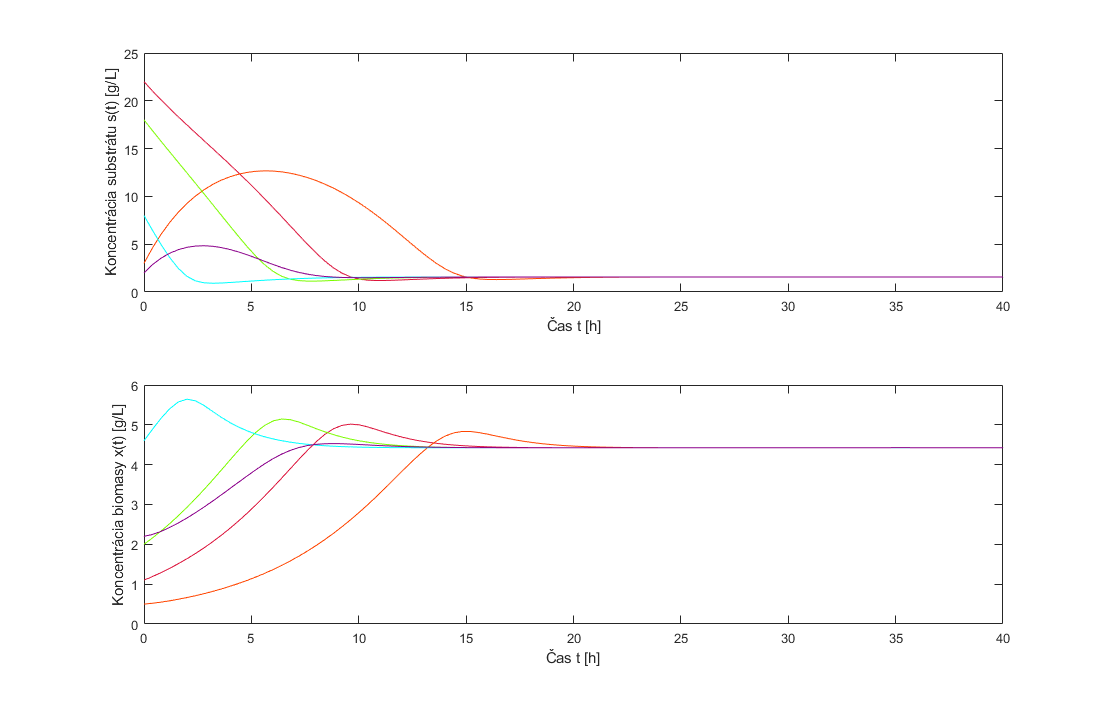
\includegraphics[width=1\linewidth]{images/init_cond_Monod}
		\caption[]{Časový priebeh koncentrácie substrátu a biomasy.}
	\end{subfigure}
	\begin{subfigure}{.5\textwidth}
		\centering
		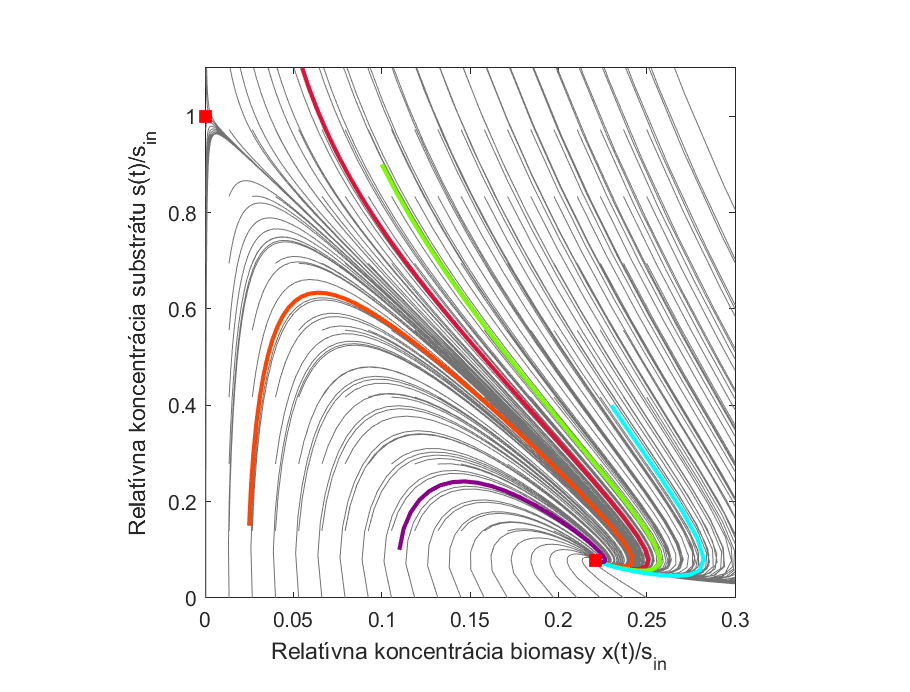
\includegraphics[width=1\linewidth]{images/phase_Monod}
		\caption[]{Fázový diagram.}
	\end{subfigure}
	\caption{Stabilita a ustálený stav Monod modelu pri nastavení parametrov uvedených v Tabuľke \ref{tab: 3}.}
	\label{fig:4}
\end{figure}

Na  fázovom diagrame Monod modelu(Obr. \ref{fig:4} napravo), môžme vidieť oba ustálené stavy. Ak zvolíme začiatočné podmienky rôzne od nuly (najmä pri koncentrácii biomasy -- vedú k triviálnemu riešeniu a systémom bude pretekať čerstvý substrát) pri konštantnej rýchlosti riedenia menšej alebo rovnej ako špecifická rýchlosť rastu, sa vždy dostaneme do toho istého ustáleného stavu.

Model s inhibíciou vykazuje odlišné správanie. Na fázovom diagrame (Obr.\ref{fig:5} napravo) môžme sledovať už dva nenulové stavy a jeden nulový. Výsledkom triviálneho riešenia je "výplach", ktorý vedie k nulovej koncentrácii biomasy a systémom bude pretekať čerstvý substrát. Ako si môžme všimnúť, vždy keď je rýchlosť rastu biomasy pomaľšia ako je odtok suspenzie zo sýstému, dostneme sa do výplachu.

\begin{figure}
	\begin{subfigure}{.5\textwidth}
		\centering
		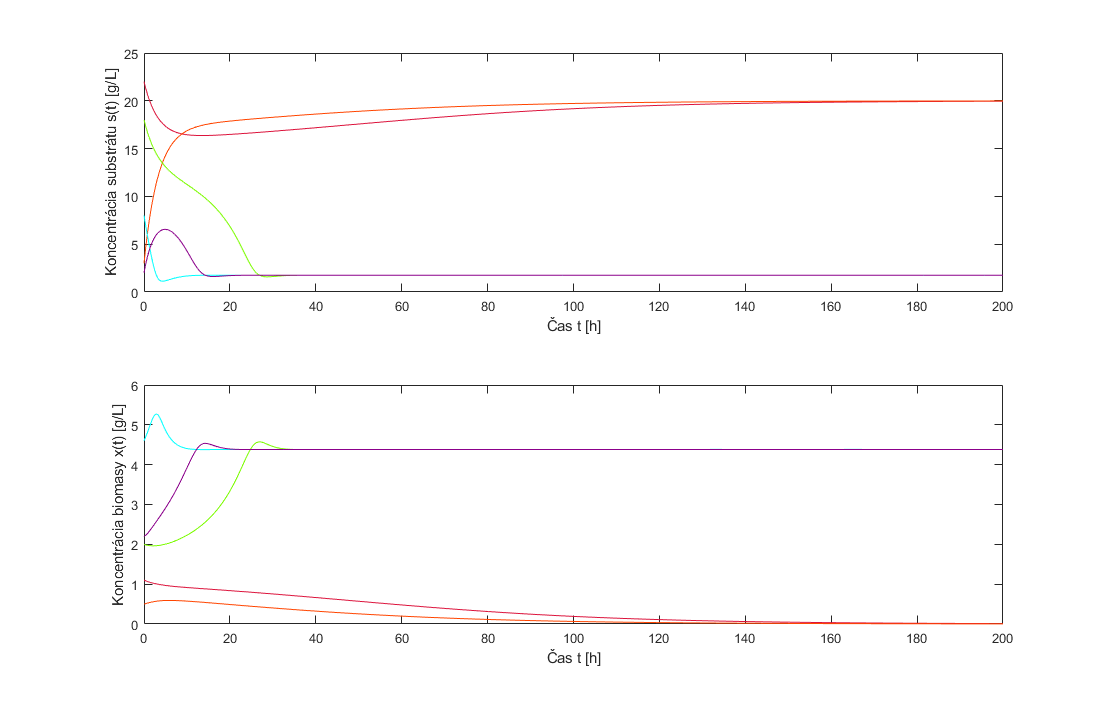
\includegraphics[width=1\linewidth]{images/init_cond_inhb}
		\caption[]{Časový priebeh koncentrácie substrátu a biomasy.}
	\end{subfigure}
	\begin{subfigure}{.5\textwidth}
		\centering
		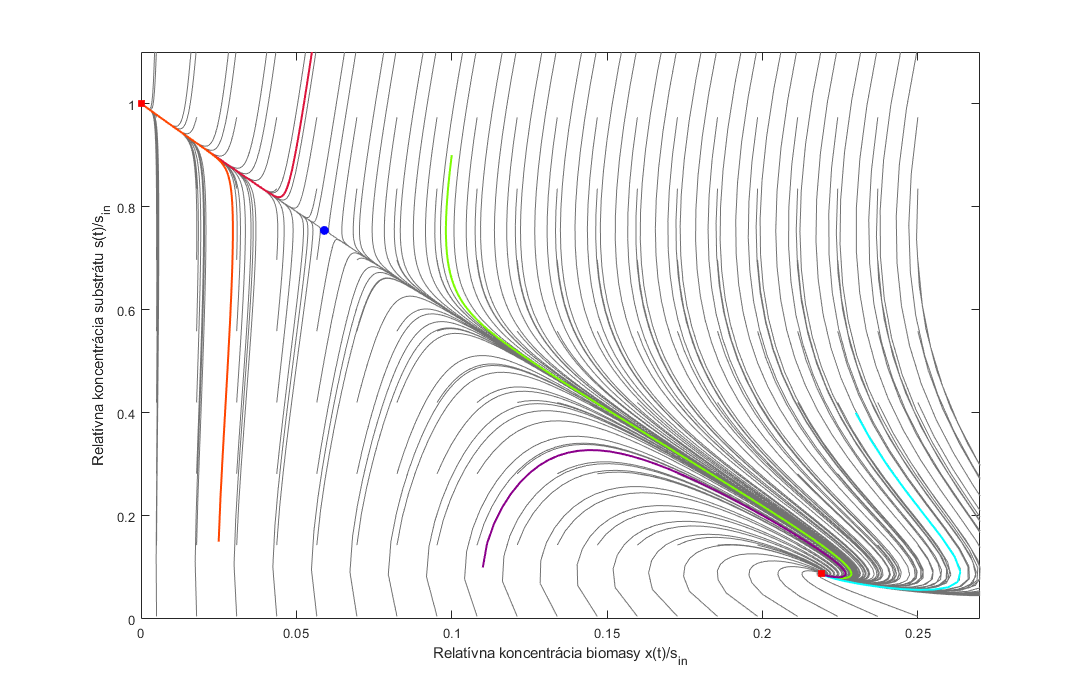
\includegraphics[width=1\linewidth]{images/phase_inhb}
		\caption[]{Fázový diagram. Červeným štvorčekom sú označené stabilné ustálené stavy, modrou guličkou je označený nestabilný stav.}
	\end{subfigure}
	\caption{Stabilita a ustálené stavy modelu s inhibíciou pri nastavení parametrov uvedených v Tabuľke \ref{tab: 3}.}
	\label{fig:5}
\end{figure}

\noindent Ostali dva netriviálne stavy, z ktorých jeden je nestabilný a druhý je stabilný. V okolí nestabilného stavu môžu nastať dva prípady a to v závislosti od počiatočných podmienok. Ak sa nachádzame na Obr. \ref{fig:2} naľavo, to znamená, že rýchlosť rastu biomasy je väčšia ako odtok suspenzie, dostaneme sa do nenulového ustáleného stavu. Ak sa nachádzame viac napravo, dostaneme sa do výplachu.

\begin{table}
	\centering
	\caption{Nastavenie parametrov Monod modelu a modelu s inhibíciou. Údaje pod čiarou mali danú veľkosť v prípade, že sa nemenili.}
	\label{tab: 3}
	\begin{tabular}{lll}
		\hline
		\textbf{Parameter} & \textbf{Veľkosť} & \textbf{Rozmer} \\
		\hline
	 	$\mu_{m}$ & 0.53 & \unitfrac{1}{\hour} \\
	 	$\nu$ & 0.5 & \unitfrac{1}{\hour} \\
		$K_{M}$ & 1.2 & \unitfrac{\gram}{\liter} \\
		$K_{i}$ & 22 & \unitfrac{\gram}{\liter} \\
		$Y_{x}$ & 0.4 & \\
		$Y_{p}$ & 1 & \\
		$V$ & 3.33 & \liter \\
		$F$ & 1 & \unitfrac{\liter}{\hour} \\
		\hline
		$s_{in}$ & 20 & \unitfrac{\gram}{\liter} \\
		$p_0, s_0$ & 0 & \unitfrac{\gram}{\liter} \\
		$x_0$ & 10 & \unitfrac{\gram}{\liter} \\
		\hline
	\end{tabular}
\end{table}

Ďalší parameter, ktorý dokáže ovplyvniť stabilitu systému, je koncentrácia čerstvého substrátu. Z Obr. \ref{fig:7} je zrejmé, že ak koncentrácia čerstvého roztoku je nižšia ako nejaká minimálna hodnota, náš systém pôjde do výplachu. Koncentrácia čerstvého substrátu ovplyvňuje špecifickú rýchlosť rastu (viď Obr. \ref{fig:2} ). Tým pádom ak sa nachádzame v oblasti pod prvým nenulovým ustáleným stavom (ten v takomto prípade neexistuje, pretože sme mimo pracovného nastavenia) dochádza k výplachu. Ak sa chceme dostať do nenulového ustáleného stavu, je nutné aby koncentrácia čerstvého substrátu bola vyššia ako koncentrácia v prvom nenulovom ustálenom stave. Pri Monod modely by sme mohli ísť s touto koncentráciou do nekonečna, kde by sme dosiahli maximálnu rýchlosť rastu. Ale na rozdiel od Monod modelu, pri modely s inhibícou, by od istého momentu ($S^{*} = \sqrt{K_M K_i}$) so zväčšujúcou sa koncentráciou čerstvého substrátu klesala špecifická rýchlosť rastu, ktorá sa limitne blíži k nule a koncentrácia biomasy padne na nulu.

\begin{figure}
	\centering
	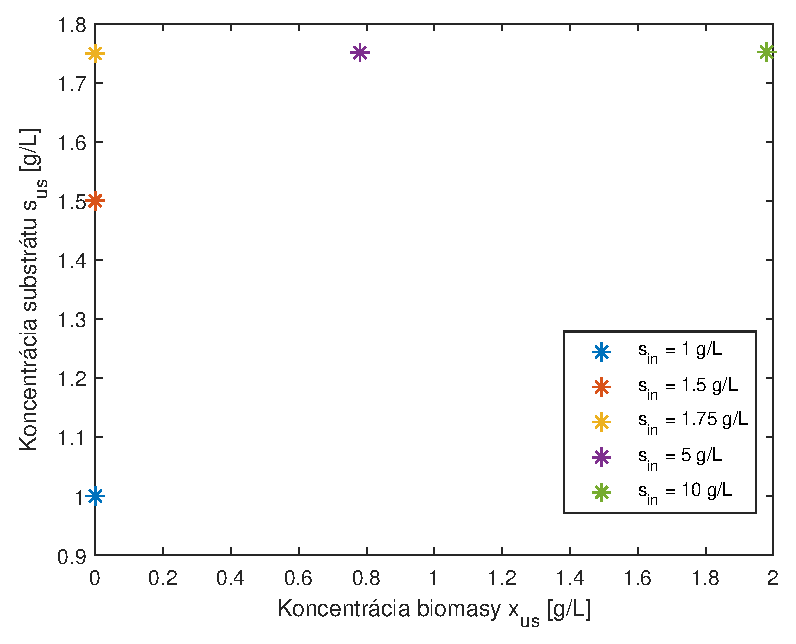
\includegraphics[width=.7\linewidth]{images/s_in_inhb}
	\caption[]{Závislosť koncentrácie substrátu od koncentrácie biomasy v ustálenom stave pri rôznych koncentráciach čerstvého substratu $s_{in}$.}
	\label{fig:7}
\end{figure}